\section{Эвристический алгоритм для улучшения сходимости} \label{ch3:heuristic}
	Рассмотрим эксперимент приведенный в \taref{tab:order-experiment} и представим (в виде графика) отношение суммы модулей функций ограничений к номеру итерации(\firef{fig:csum-over-iterations}). 

\begin{figure}[ht!] 
	\center
	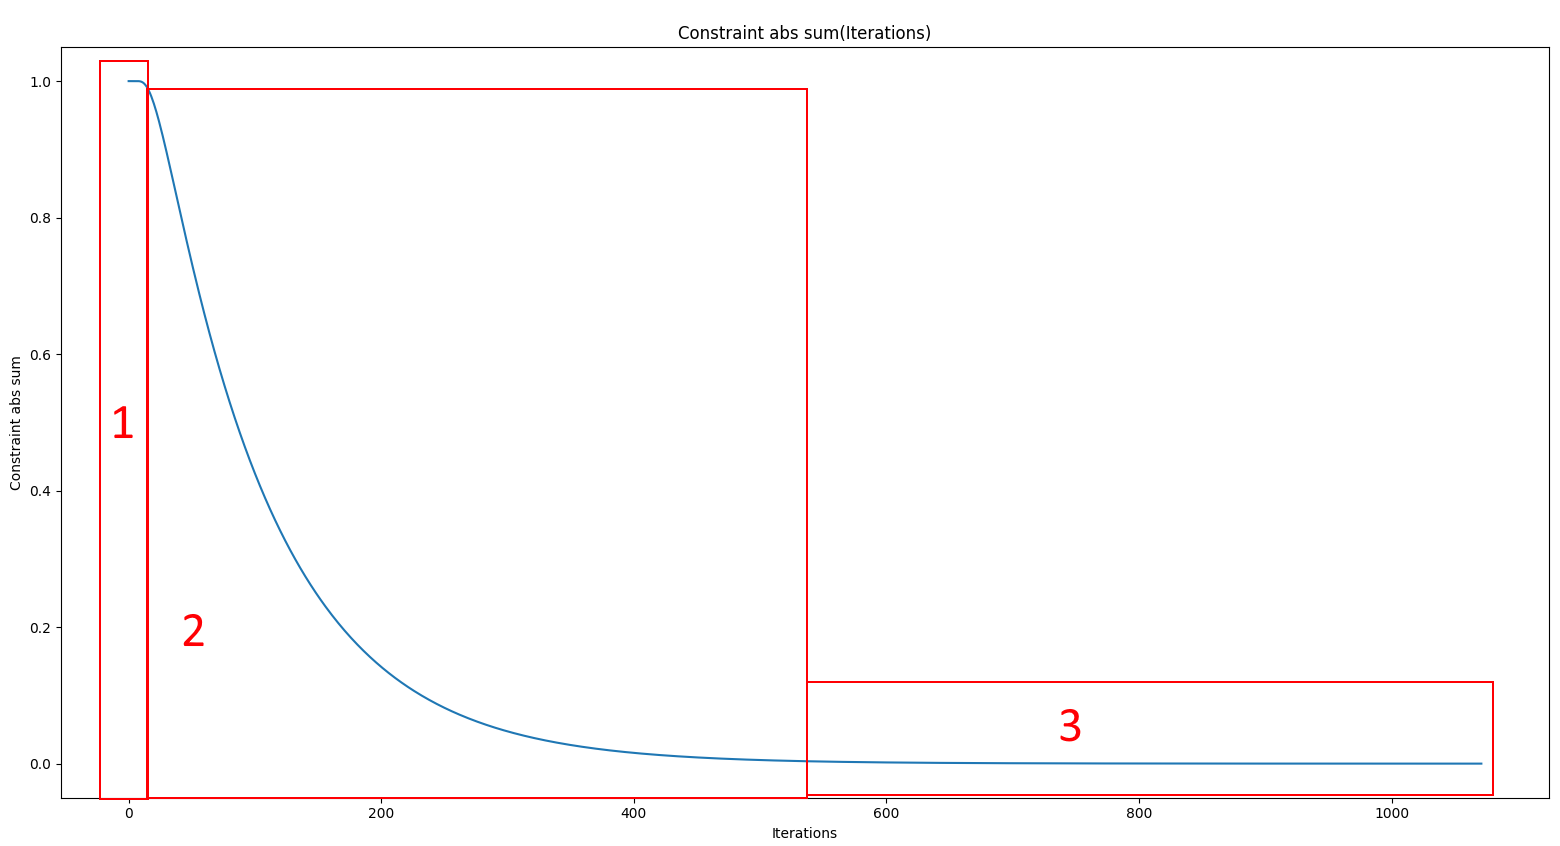
\includegraphics [scale=0.4] {my_folder/images//plot_16_coloring.png}
	\caption{Отношение суммы модулей функций ограничений к номеру итерации. Количество частиц 16, обход $coloring$.}
	\label{fig:csum-over-iterations}  
\end{figure}	

	На данном графике можно выделить 3 секции:
	\begin{enumerate}[1.]
		\item Небольшое плато в начале графика. Размер данной секции и является различной частью, при использовании обходов $forward$, $backward$ и $coloring$.
		\item Резкий спад. На данном этапе \say{снимается}  наибольшее растяжение.
		\item Большое плато, в котором достигается необходимая точность.
	\end{enumerate}

	Исходя из данного графика, можно заметить, что наибольшее число итераций занимают именно секции 2 и 3. Рассмотрим(\taref{tab:constarint-values}) значения функций ограничений на некоторых итерациях алгоритма PBD, рассматривая при этом обход $forward$, так как для него секция 1 отсутствует.
	
	\noindent % for correct centering
	\begin{minipage}{\textwidth}
		\vspace{\mfloatsep} % интервал 
		\centering\small
		\captionof{table}{Значения функций ограничений для одномерной веревки (8 частиц) на различных итерациях алгоритма PBD обходе $forward$)}%
		\label{tab:constarint-values}
		\begin{tabular}{|c|c|c|c|c|c|c|c|c|}
			\hline
			\textbf{Итерация} & $\mathbf{\sum_{i = 1}^{7}|C_i|}$ & $\mathbf{|C_1|}$ & $\mathbf{|C_2|}$ & $\mathbf{|C_3|}$ & $\mathbf{|C_4|}$ & $\mathbf{|C_5|}$ & $\mathbf{|C_6|}$ & $\mathbf{|C_7|}$ \\
			\hline
			$\mathbf{0}$ & $1.0$ & $1.0$ & $0.0$ & $0.0$ & $0.0$ & $0.0$ & $0.0$ & $0.0$ \\ \hline
			$\mathbf{1}$ & $0.984375$ & $0.5$ & $0.25$ & $0.125$ & $0.0625$ & $0.03125$ & $0.015625$ & $0.0$ \\ \hline
			$\mathbf{2}$ & $0.957031$ & $0.375$ & $0.25$ & $0.15625$ & $0.09375$ & $0.054687$ & $0.027343$ & $0.0$ \\ \hline
			$\mathbf{3}$ & $0.922851$ & $0.3125$ & $0.234375$ & $0.1640625$ & $0.109375$ & $0.068359$ & $0.034179$ & $0.0$ \\ \hline
			$\mathbf{4}$ & $0.885253$ & $0.273437$ & $0.21875$ & $0.164062$ & $0.116210$ & $0.075195$ & $0.037597$ & $0.0$ \\ \hline
			$\mathbf{5}$ & $0.846374$ & $0.246093$ & $0.205078$ & $0.160644$ & $0.117919$ & $0.077758$ & $0.038879$ & $0.0$ \\ \hline
			$\mathbf{10}$ & $0.662745$ & $0.174022$ & $0.155377$ & $0.130353$ & $0.100749$ & $0.068161$ & $0.034081$ & $0.0$ \\ \hline
			$\mathbf{20}$ & $0.399291$ & $0.103489$ & $0.093230$ & $0.078865$ & $0.061312$ & $0.041595$ & $0.020797$ & $0.0$ \\ \hline
			$\mathbf{50}$ & $0.087025$ & $0.022551$ & $0.020318$ & $0.017189$ & $0.013364$ & $0.009067$ & $0.004533$ & $0.0$ \\ \hline
			$\mathbf{100}$ & $0.006869$ & $0.001780$ & $0.001603$ & $0.001356$ & $0.001054$ & $0.000715$ & $0.000357$ & $0.0$ \\ \hline
			$\mathbf{200}$ & $0.000042$ & $0.000011$ & $0.000009$ & $0.000008$ & $0.000006$ & $0.000004$ & $0.000002$ & $0.0$ \\ \hline
			$\mathbf{229}$ & $0.000009$ & $0.000002$ & $0.000002$ & $0.000001$ & $0.000001$ & $0.000001$ & $0.000001$ & $0.0$ \\ \hline
		\end{tabular}
		\vspace{\mfloatsep} % интервал 
		\normalsize %восстанавливаем шрифт 	
	\end{minipage} 
	
	Исходя из полученных значений заметим:
	\begin{enumerate}[1.]
		\item После первой итерации значения модулей функций ограничения, совпадают с элементами последовательности $\{\frac{1}{2^n}\}$.
		\item После первой итерации суммарное значение модулей функций ограничения, уменьшилось на $\frac{1}{64} =\frac{1}{2^8}$.
		\item После каждой итерации значение модуля функции 7-ого ограничения всегда равно $0.0$. 
		\item Наибольшая скорость сходимости наблюдается тогда, когда значения модулей ограничения близки друг к другу.
	\end{enumerate}

	В связи с наблюдением 4. возникает желание \say{разравнять} значения функциий растяжения между собой так, чтобы увеличить скорость сходимости. Для этого, попробуем ещё раз запустить этот эксперимент, однако раз в $HeuristicStep$ итераций, помимо обхода ограничений будем запускать алгоритм представленный на \firef{alg:Heuristic1D}.
	
	\begin{algorithm} %[h]
		\SetKwFunction{algoHeuristicOneDimPseudocode}{} 
		\SetKwProg{myalg}{Algorithm}{}{} %write in 2nd agrument <<Algorithm>>, <<Procedure>> etc
		\nonl\myalg{\algoHeuristicOneDimPseudocode}{
			\KwInput{
				количество частиц $N$,
				предсказанные положения частиц $p^*_i$,
				параметр интерполяции $HeuristicAlpha$
			}
			\KwOutput{новые положения частиц $p^*_i$}
			
			$ropeLength = |p^*_N - p^*_1|$
			
			$ropeDir = \frac{p^*_N - p^*_1}{ropeLength}$
			
			\For {$\forall p^*_i $}{
				$lengthFromStart = \frac{i-1}{N-1} * ropeLength$

				$p'_i = p^*_1 + ropeDir * lengthFromStart$ 
								
				$p^*_i = p^*_i * (1 - HeuristicAlpha) + p'_i * (HeuristicAlpha)$;
			}
		}
		\caption{Псевдокод эвристического алгоритма для веревки в одномерном пространстве}\label{alg:Heuristic1D}
	\end{algorithm}
	\FloatBarrier
	
	На \firef{fig:heuristicPlotAlpha} \firef{fig:heuristicPlotStep} представлено отношение суммарного значения модулей функций ограничения к номеру итерации для разных значений $HeuristicStep$ и $HeuristicAlpha$. 
	
	\begin{figure}[ht!] 
		\center
		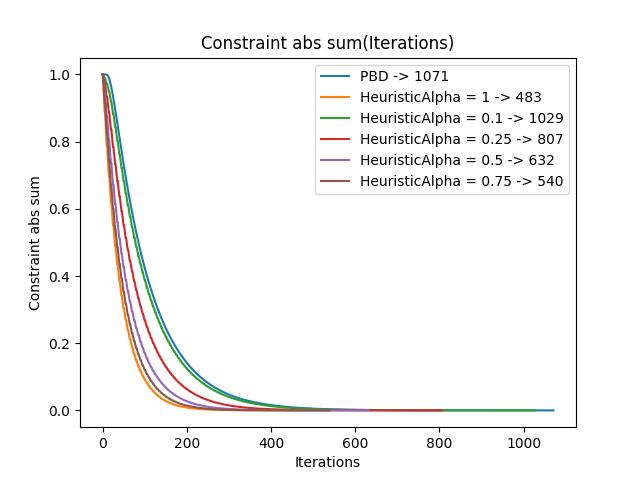
\includegraphics [scale=0.4] {my_folder/images//heuristicPlotAlpha.png}
		\caption{Отношение суммы модулей функций ограничений к номеру итерации с использованием эмпирического алгоритма. Количество частиц 16, обход $coloring$, $HeuristicStep=5$. В легенде обозначено итоговое количество итераций}
		\label{fig:heuristicPlotAlpha}  
	\end{figure}
	\FloatBarrier
	
	\begin{figure}[ht!] 
		\center
		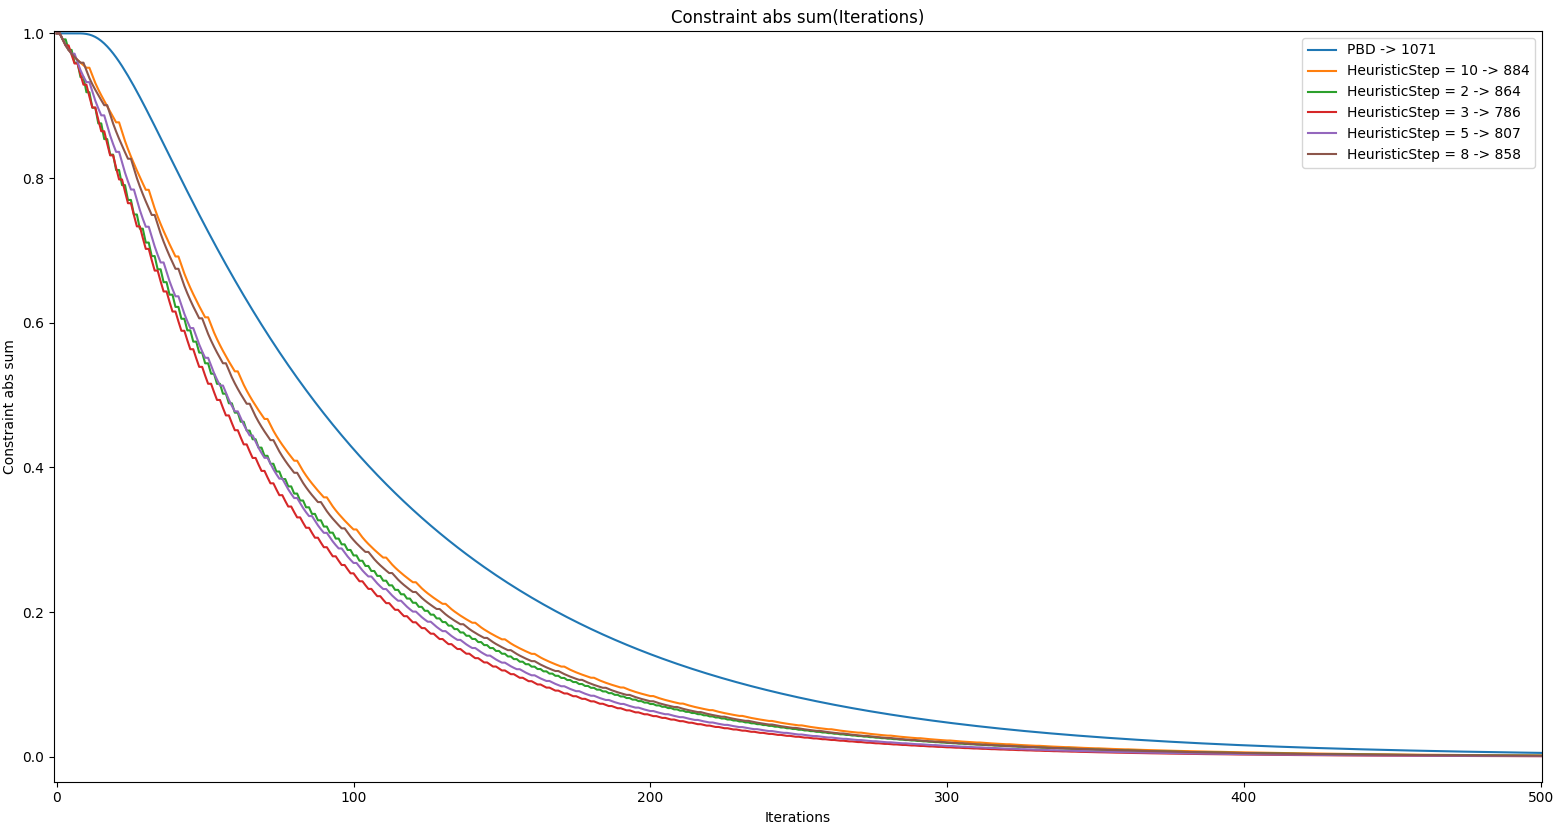
\includegraphics [scale=0.4] {my_folder/images//heuristicPlotStep.png}
		\caption{Отношение суммы модулей функций ограничений к номеру итерации с использованием эмпирического алгоритма. Количество частиц 16, обход $coloring$, $HeuristicAlpha=0.25$. В легенде обозначено итоговое количество итераций}
		\label{fig:heuristicPlotStep}  
	\end{figure}	
	\FloatBarrier
	
	Таким образом можно сделать вывод что предлагаемый алгоритм работает и количество итераций действительно снизилось. Данный алгоритм можно рассматривать как итерацию к удовлетворению условию \ref{eq:heurV1Idea}, которое напрямую вытекает из \ref{eq:constraint-eq} и означает равенство \say{плотностей}.
	
	\begin{equation} \label{eq:heurV1Idea}
		\forall i,j : C_i(p) = C_j(p) = \frac{\sum_k^M C_k(p)}{M}
	\end{equation}
	
	Однако данный алгоритм имеет ряд недостатков:
	\begin{enumerate}[1.]
		\item Данный алгоритм(\firef{alg:Heuristic1D}) применим только в одномерном случае
		\item Он применим только для алгоритма PBD 
		\item Он применим только в случае бесконечной жесткости
		\item Он применим только для веревок
		\item Данный алгоритм модифицирует положения частиц не используя значения ограничений, связывающие их. Из-за этого, на этапе вычисления скоростей частиц будет внесена ошибка, приводящая к заметным колебаниям.
	\end{enumerate}
	
	Для решения недостатка под пунктом 1, перестроим алгоритм так, чтобы вместо длин в пространстве он оперировал длинами вдоль веревки. Для этого нам будет необходимо посчитать префиксную сумму длин для веревки. Затем, найти $lengthFromStart$ - расстояние (вдоль веревки) от первой частицы до $p'_i$. Далее, при помощи префиксной суммы можно определить, между какими двумя частицами $p^*_j$ и $p^*_{j+1}$  находится $p'$. И наконец, найти $p'$ при помощи линейной интерполяции.
	
	На \firef{fig:heuristicSchema} представлено расположение точек при использовании данной идеи.
	
	\begin{figure}[ht!] 
		\center
		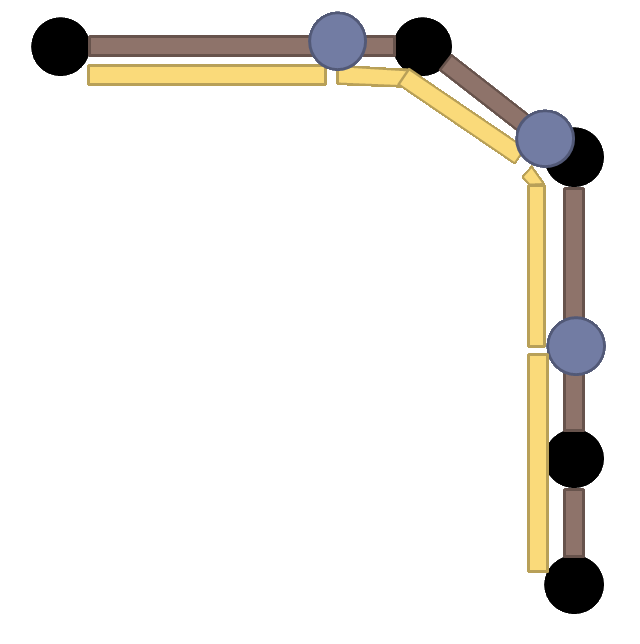
\includegraphics [scale=0.4] {my_folder/images//heuristicSchema}
		\caption{Графическое представление идеи эвристическго алгоритма. Черным представлены точки $p^*_i$, коричневым - ограничения их соединяющие. Синим представлены точки $p'_i$ используемые в алгоритме, а желтым показаны секции с равной длиной вдоль веревки}
		\label{fig:heuristicSchema}  
	\end{figure}	
	\FloatBarrier 
	
	Описанный эвристический алгоритм можно также рассматривать как построение кривой по опорным точкам, с последующим выбором новых опорных точек. Результатом данного \say{ресемплинга} не всегда будет та же самая кривая (как показано на \firef{fig:heuristicSchemaFail}), однако используя параметры $HeuristicAlpha$ и $HeuristicStep$ можно контроллировать величину допускаемого отклонения. Помимо этого стоит отметить, что при большой плотности частиц данные ситуации маловероятны.
	
	\begin{figure}[ht!] 
		\center
		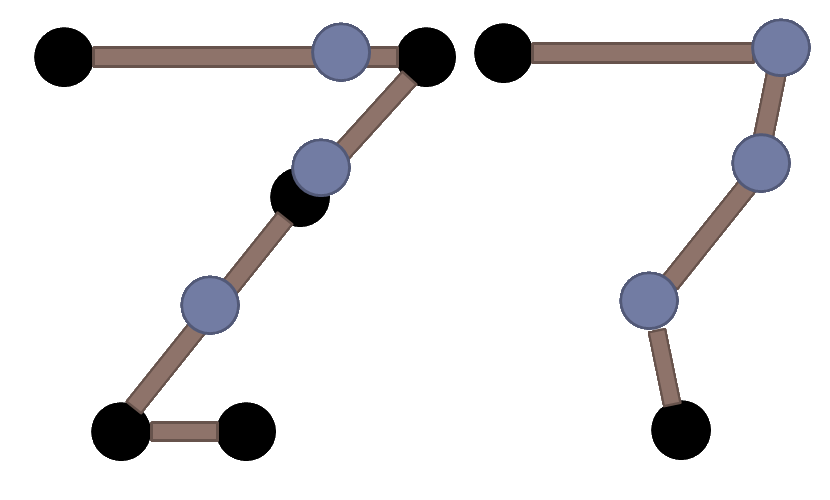
\includegraphics [scale=0.4] {my_folder/images//heuristicSchemaFail}
		\caption{Графическое представление ошибок эвристическго алгоритма при $HeuristicAlpha = 1$. Слева представлена конфигурация до применения эвристического алгоритма, справа после. Черным представлены точки $p^*_i$, коричневым - ограничения их соединяющие. Синим представлены точки $p'_i$ используемые в алгоритме.}
		\label{fig:heuristicSchemaFail}  
	\end{figure}	
	\FloatBarrier 
	
	Для решения недостатков связанного с применимостью только для алгоритма PBD, а также бесконечной жесткости, перепишем выражение \ref{eq:xpbd_second} в стиле выражения \ref{eq:heurV1Idea}. Тогда мы получим:
	
	\begin{equation} \label{eq:heurV2Idea}
		\forall i,j : C_i(p) + \frac{\alpha}{\delta t^2}\lambda_i = C_j(p) + \frac{\alpha}{\delta t^2}\lambda_j = \frac{\sum_k^M C_k(p) + \frac{\alpha}{\delta t^2}\lambda_k}{M}
	\end{equation}
	
	В данном выражении мы не знаем $\lambda_k$, однако, используя подход Small steps описанный в главе \ref{ch2:xpbd}, мы можем приравнять $\lambda_k$ к $\delta \lambda_k$, которые можем найти при помощи \ref{eq:xpbd-delta-lambda-2}. Используя в данном алгоритме вместо суммы длин, сумму величин приведенных в \ref{eq:heurV2Idea}, мы делаем возможным применение эвристического алгоритма вместе с XPBD, и разными значениями жесткости.
	
	Для решения недостатка связанного с обсчётом скоростей на следующем шаге итерации, необходимо (применяя технику Small Steps) вынести применение эмпирического алгортма из цикла обработки ограничений, поставив его перед интегрированием скоростей. Затем, модифцировать значения положений прошлой итерации таким образом, чтобы скорости проинтерполировались соответственно проинтерполированным значениям (всё также используя идею \say{ресемплинга}).
	
	Для решения последней проблемы, связанной с тем что данный метод применим только к веревкам, вспомним (глава \ref{ch2:pbd-improvments}), что основным подходом для расставления ограничений является задание поверхности ткани в виде прямоугольной сетки. Тогда рассмотрим строки этой сетки, получающиеся при соединении частиц горизонтальными и вертикальными структурными ограничениями. Данные строки являются веревками, а значит к ним также применим эврестический метод. При этом стоит отметить, что веревки одной ориентации могут быть обработаны параллельно между собой(\firef{fig:ropesInCloth}).
	
	\begin{figure}[ht!] 
		\center
		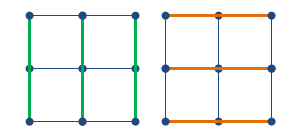
\includegraphics [scale=0.8] {my_folder/images//bending}
		\caption{Визуальная демонстрация расположения веревок для ткани размероности 3 на 3 частицы}
		\label{fig:ropesInCloth}  
	\end{figure}
	
	Применив все вышеописанные улучшения, мы получаем эмпирический алгоритм представленный на \firef{alg:HeuristicV2}.
	
	\begin{algorithm} [h]
		\SetKwFunction{ImprovedHeuristicAlgorithm}{} 
		\SetKwProg{myalg}{Algorithm}{}{} %write in 2nd agrument <<Algorithm>>, <<Procedure>> etc
		\nonl\myalg{ImprovedHeuristicAlgorithm}{
			\KwInput{
				время шага симуляции $\delta t$,
				текущие положения частиц $p_i(t)$,
				предыдущие положения частиц $p_i(t - \delta t)$,
				обратные масссы частиц $im_i$,
				обратная жесткость $\alpha$,
				параметр $HeuristicAlpha$
			}
			\KwOutput{обновленные положения частиц $p_i(t)$, $p_i(t - \delta t)$ }
			
			Заполнение массива $lengths$ как префиксную сумму величин $|p_i(t) - p_{i+1}(t)|$
			
			Заполнение массива $coeffs$ как префиксную сумму величин $C_i(p_i(t), p_{i+1}(t)) + \delta \lambda_i$			
			
			$totalLength = lengths[N-1]$
			
			$totalCoeff = coeffs[N-1]$
			
			\For {$\forall i \in 2..N-1 $}{
				
				$lengthFromStart = totalLength * coeffs[i] / totalCoeff$
				
				Бинарный поиск j такого что $lengths[j-1] $\leq$ lengthFromStart < lengths[j]$ 
				
				$t = \frac{lengthFromStart - lengths[j-1]}{lengths[j] - lengths[j-1]}$
				
				$p'_i = p_{j-1}(t) * (1 - t) + p_j(t) * t$
				
				$v'_i = \frac{p_{j-1}(t) - p_{j-1}(t - \delta t)}{\delta t} * (1 - t) + \frac{p_{j}(t) - p_{j}(t - \delta t)}{\delta t} * t$
				 
				$v_i = \frac{p_i(t) - p_i(t - \delta t)}{\delta t}$
				 
				$p_i(t) = p_i(t) * (1 - HeuristicAlpha) + p'_i * (HeuristicAlpha)$;				

				$v_i = v_i * (1 - HeuristicAlpha) + v'_i * (HeuristicAlpha)$
				
				$p_i(t - \delta t) = p_i(t) - v_i * \delta t$
			}
		}
		\caption{Псевдокод эвристического алгоритма для веревки в многомерном пространстве с поддержкой XPBD и обработкой скоростей}\label{alg:HeuristicV2}
	\end{algorithm}
	
	А соответствующий ему алгоритм Extended Position Based Dynamics, в котором применена техника Small Steps и показано как именно встраивается в его работу эврестический алгоритм, представлен на \firef{alg:HeuristicXPBD}
	
	\begin{algorithm} [h]
		\SetKwFunction{algoXPBDSmallStepsPseudocode}{} 
		\SetKwProg{myalg}{Algorithm}{}{} %write in 2nd agrument <<Algorithm>>, <<Procedure>> etc
		\nonl\myalg{\algoXPBDSmallStepsPseudocode}{
			\KwInput{
				время шага симуляции $\delta t$,
				количество шагов $solverStep$,
				количество итераций $solverIteration$,
				текущее состояние частиц,
				предыдущее состояние частиц,
				ограничения,
				функция суммы внешних сил $f_{ext}(p)$,
				параметр $HeuristicStep$,
				параметр $HeuristicAlpha$
			}
			\KwOutput{положение частиц спустя заданное время $p_i(t + \delta t)$}
			
			$stepT = \delta t / solverStep$;
			
			\For{$\forall step \in 1..solverStep$}{
				
				\If{$mod(step, HeuristicStep) = 0$}
				{
					\lFor{horizontal rope}
					{
						$HeuristicAlgorithm()$
					}
					
					\lFor{vertical rope}
					{
						$HeuristicAlgorithm()$
					}
				}
				
				Произвести шаг XPBD в соответствии c \firef{alg:ExtendedPositionBasedDynamicsSmallSteps}
			}
		}
		\caption{Псевдокод алгоритма Extended Position Based Dynamics с использованием эвристического алгоритма }\label{alg:HeuristicXPBD}
	\end{algorithm}
	\FloatBarrier
	
%% Вспомогательные команды - Additional commands
%
%\newpage % принудительное начало с новой страницы, использовать только в конце раздела
%\clearpage % осуществляется пакетом <<placeins>> в пределах секций
%\newpage\leavevmode\thispagestyle{empty}\newpage % 100 % начало новой страницы